\chapter{\uppercase{Design}}

This chapter focusses on the overall architecture of Xen and its modifications.
\section{Xen Architecture}

Xen is an open-source hypervisor, which started as a project at University of Cambridge. Since x86 ISA was not natively virtualizable, Xen was only compatible with specific modified Linux kernel versions. With increasing popularity of the hypervisor, these changes were incorporated in the mainstream Linux kernel.

In a Xen based system, memory and CPU resources are managed directly by the hypervisor, but I/O devices are generally controlled using privileged VM, generally Domain0. This domain runs in a privileged mode where it has direct access to the bare hardware resources. In addition to handling I/O operations, it also hosts the Xen User Interface which is used to administer commands to the hypervisor.



\begin{figure}
\centering
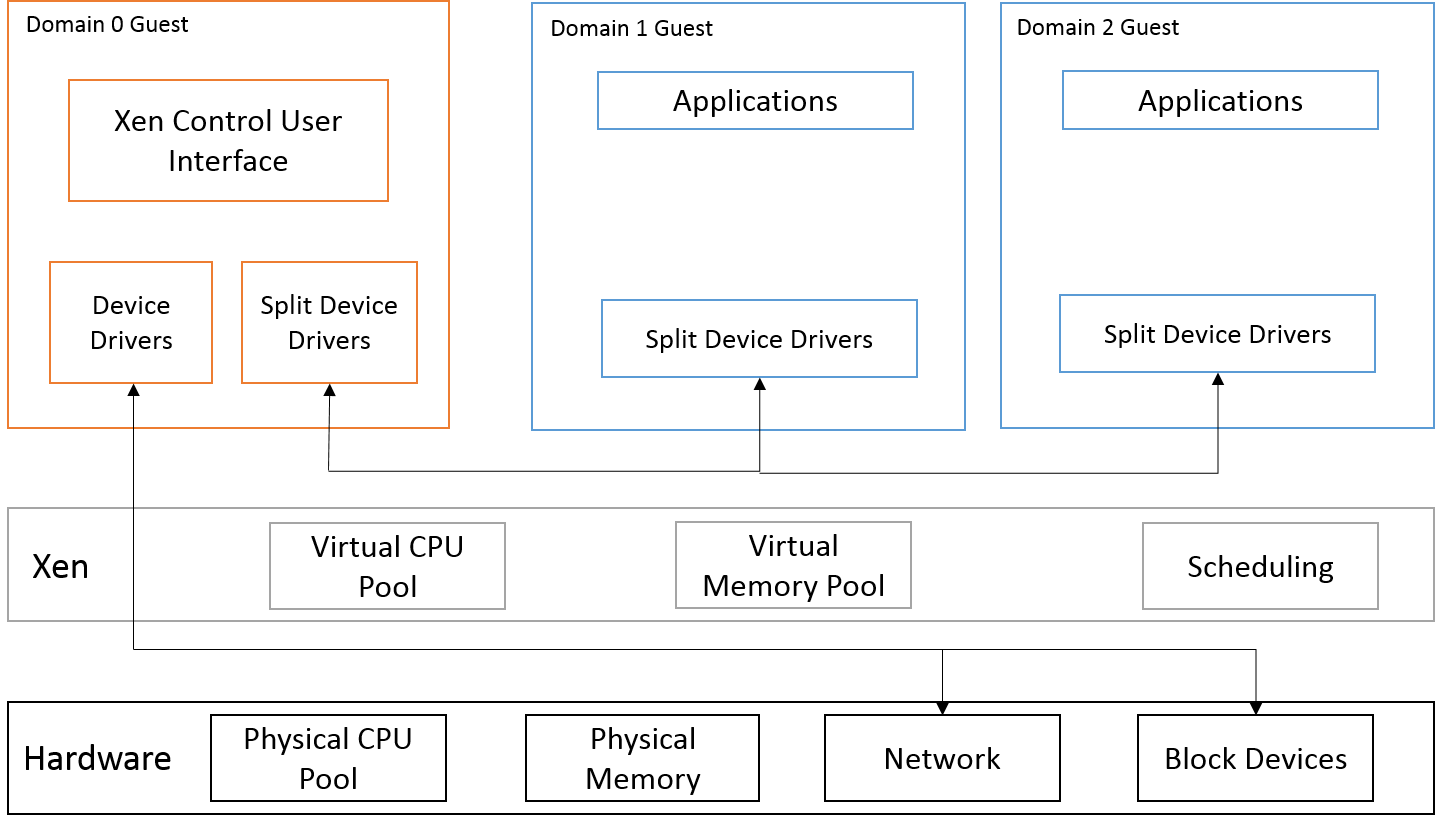
\includegraphics[scale=0.6]{figures/Xen_model.png}
\caption{Xen Architecture}
\label{fig:xen_model}
\end{figure}

Similar to the usage of system calls by applications, Linux uses hypercalls to request resources and pass over control to the hypervisor. The hypervisor in turn communicates with the Linux kernel via event channels.

One of the features of Xen which makes it very popular is the I/O interface. With Domain 0 hosting the device drivers, Xen escapes the need to both emulated the device and and develop separate drivers. If a Guest Domain needs to perform an I/O operation, only the specifics and data need to be forwarded to the Domain 0. This is accomplished via a generic split device driver model. A generic front end device driver is installed in the guest domain, which captures the I/O request specifics and forwards it to the back-end device driver present in Domain0. The

backend device driver then decodes the I/O requests and forwards it to the real device driver. A key advantage is that a split device driver is not device specific, it covers a whole class devices.

Virtual machines in Xen have various configurable parameters which are defined in a config file. This file typically indicates, disk storage location, required memory, attached I/O devices, virtual CPUs’ required etc. A virtual machine is powered on and off using the Xen User Interface commands present in Dom0.


\section{Xen Memory Model}

Memory management is one of the core components of a hypervisor. With Xen core, the available memory is shared dyanamically amongst the different virtual machines. It also allows for thin provisioning, i.i. projecting more memory than the available physical RAM using ballooning techniques.

As a part of design philosophy, Xen does not swap pages out of memory itself. Individual guest OSes’ are the best judges to identify cold pages and thus this job is left over to them. Using the balloon driver, Xen is able to mount or release memory pressure in a VM. When the hypervisor wants to reclaim pages from a VM, it inflates the balloon driver in the virtual machine. The balloon driver requests more memory from the OS, which swaps cold pages out and releases memory to the balloon driver. The latter in turn, returns those freed up memory pages to the hypervisor which can allocate to the appropriate VM. During runtime, as the memory requirement is released, Xen deflates the balloon and releases memory back to the VM.

Memory Mapping

A virtual address space is generally divided into two parts

1. Kernel Space: This space is shared and common to all the applications. Kernel space also contains a direct mapping of the physical address space (usually with an offset).

2. Application Space: This space is specific to individual applications for application data and code.

32-bit Linux machines have a 3GB/1GB split, where the lower 3GB is occupied by the application. 64-bit x86 machines on the other hand only allow 48-bit signed addresses, in which the lower segment goes to the application and the upper segment is occupied by the kernel. Mapping the kernel into the individual application address spaces avoids the overhead of a context switch during a system call.

Insert pictures of address spaces here.

A similar framework is setup in-between Xen hypervisor and the individual VMs, where Xen occupies a small part of the virtual address space to avoid context switch overhead during hypercalls. The memory layout is present below:

INSERT table here for memory layout of XEN




A config file for a VM has two key memory parameters

1. Static max: It dictates the total guest physical address space of the VM.

2. Taget mem: This is indicative of the operational memory requirement of the VM and the balloon driver will generally try to balance the available system memory to this value.



\section{Xen Boot Procedure}
On system start, Xen boots up first to take stock of the hardware present. It first queries the BIOS of the E820 Memory map.Identifying the available  memory regions, Xen builds preliminary page tables and turns on paging mode. With paging enabled, the hypervisor can access the entire address space. It follows by building the free page lists. Each machine page is identified by a data structure called page\_struct. This structure contains runtime administrative information about the machine page such as, status, domain identifier, special page status, order, etc. An array of these structure are initialized for all the machine pages. 
 
The next job is to build a buddy system allocator data structure arranging all the pages by MEMZONE and ORDER. Here MEMZONE divides the entire machine address space in terms of the position of the first non-zero bit. It is necessary for special DMA memory requests for devices with fewe address bits. In each ZONE the pages are sorted by the order of the contiguous available pages with a maximum of 1GB. 
 
Memory requests are honoured at page granularity by accessor functions, which manipulate the above data structure following buddy system allocation. Pages returned by any doamin are first scrubbed clean of all information and added to the pool, protecting the security across domains. The pool is always  aggregated to the highest order on return requests. Direct mapping from a virtual address spae to the machine addresses make these tasks a lot simpler. 
 
Once the memory pool is ready Domain 0 is given appropriate memory regions and the kernel image is copied. the hypervisor follows to build a CPU pool out of the available cores. It initializes interrupts and other data structures and hands control over to Domain0 Linux kernel, which now initializes all the I/O devices using appropriate drivers. 



\subsection{Modifications}

To enable sharing NVRAM acrsoss separate VMs, we have to first recognize it as memory. Currently the firmware (BIOS) marks the memory region with code 90. Due to lack of standardization, this code is not recognized by Xen, and thus it treats the address space as a memory mapped I/O device. Xen inhibits from either writing to, or reading from this region. 
 
The first task would be to recognize the memory region, and mark it as Non-Volatile RAM. A separate codeword is added to the list of recognized E820 codes, to that effect. 



\section{DomU Boot Procedure}
k
aasals

\subsection{Modifications}


Insert sample text here





